
%(BEGIN_QUESTION)
% Copyright 2015, Tony R. Kuphaldt, released under the Creative Commons Attribution License (v 1.0)
% This means you may do almost anything with this work of mine, so long as you give me proper credit

This multi-voltage motor has been configured to operate on a power supply voltage of 480 VAC:

$$\includegraphics[width=15.5cm]{i03249x01.eps}$$

Calculate the amount of current through each individual winding of this motor, assuming a mechanical power output of 18.3 horsepower at an efficiency of 91\%.  Assume a power factor of 1 (unity).

\vskip 10pt

Also, calculate the expected voltage drop between terminals 1 and 4 on the motor while it is running.

\vfil 

\underbar{file i03249}
\eject
%(END_QUESTION)





%(BEGIN_ANSWER)

This is a graded question -- no answers or hints given!

%(END_ANSWER)





%(BEGIN_NOTES)

A motor outputting 18.3 HP at an efficiency of 91\% must consume 20.11 HP worth of electrical power.  This is equivalent to 15002 watts.  A common problem area for students when working with efficiency calculations is multiplying when they should divide, or vice-versa.  What needs to be borne in mind here is that any machine operating at less than 100\% efficiency (which is {\it any} real machine) must input more useful power than it outputs.  In other words, this electric motor only converts 91\% of the electrical energy given to it into mechanical work, with the remainder of 9\% converted into heat, noise, air movement, vibrations, etc.  Therefore, we must expect the electrical power value to exceed the given mechanical output power value of 18.3 HP (i.e. $P_{in} = {P_{out} \div 91\%}$).  If we were given the electrical input power value instead, then our calculated mechanical power would be a lesser quantity (i.e. $P_{out} = P_{in} \times 91\%$).

\vskip 10pt

Line current for a motor consuming 15 kW of power at 480 volts (3-phase) is equal to:

$$P_{total} = \sqrt{3} V_{line} I_{line}$$

$$I_{line} = {P_{total} \over \sqrt{3} V_{line}}$$

$$I_{line} = {15002 \over \sqrt{3} (480)} = 18.04 \hbox{ amps}$$

Delta-connected elements experience full line voltage, but carry only a fraction of the line current.  In this case, the line current of 18.04 amps will be divided by $\sqrt{3}$ to yield a phase current value of 10.42 amps through each winding inside the motor.

\vskip 10pt

The voltage drop between terminals 1 and 4 should be exactly half of the line voltage since the winding between terminals 1 and 4 comprises one-half of a winding pair in that phase of the delta connection.  Thus, each half of the winding pair sees one-half of the 480 VAC line voltage, or 240 VAC.

%INDEX% Pictorial circuit review (3-phase motor connections)

%(END_NOTES)


